\addcontentsline{lof}{chapter}{Tillegsfigurer}
\chapter{Prototyper}
I dette avsnitt blir det nærmere presentert bilder av prototyper. Hensikten er at vi ønsker å presenter bildene i bedre kvalitet enn hva som tillates inne i rapporten. Derfor valgte vi å plassere disse i spesill appendiks.
\section{Low-fi prototype} \label{sec:appendiksLowFi}
%Bredde for low-fi prototyper
\newcommand{\lowB}{0.9}
%KONFIGURASJON AV APACHE
\begin{figure}[ht]
\centering
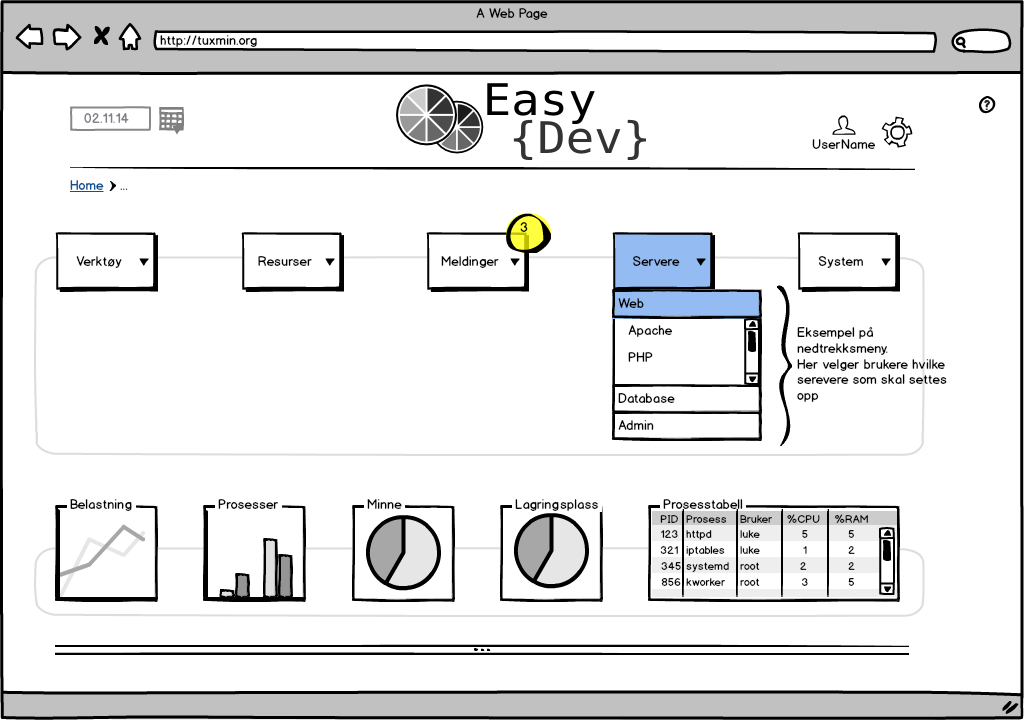
\includegraphics[width=\lowB\textwidth,height=\textheight,keepaspectratio]
{./img/prosessdokumentasjon/lowfi/apache1.png}
\caption[Low-fi Webserver 1]{Webserver. Her sakl brukeren sette igang konfigurasjon av webserver. Modulen for dette er logisk plassert under <<Servere>> kategorien.}
\label{fig:apachelow1}
\end{figure}

\begin{figure}[ht]
\centering
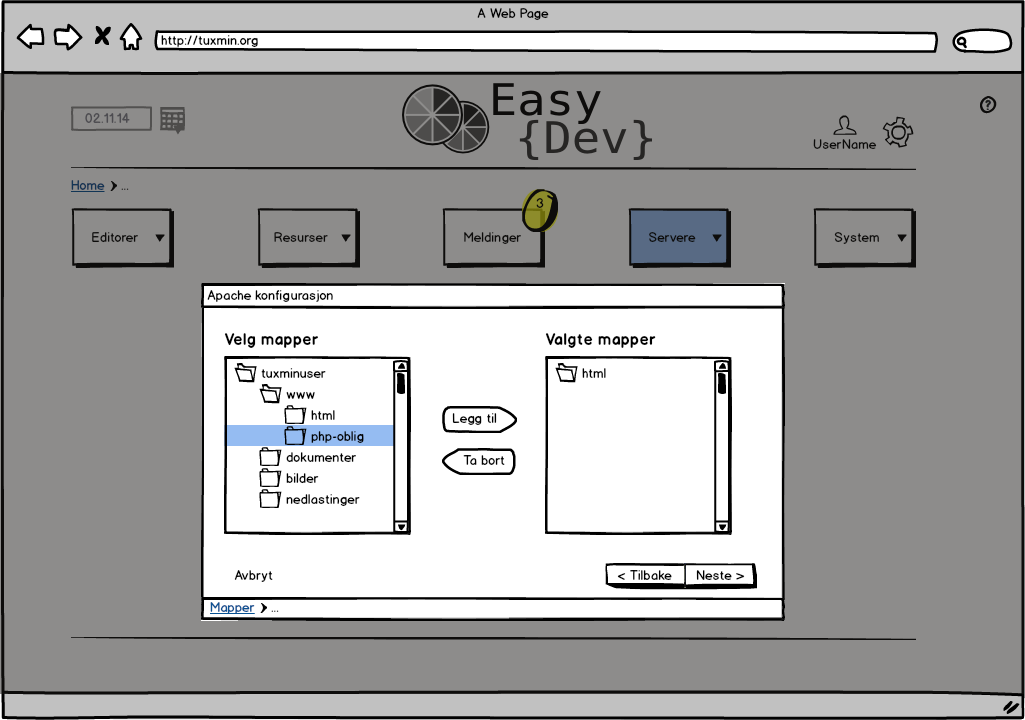
\includegraphics[width=\lowB\textwidth,height=\textheight,keepaspectratio]{./img/prosessdokumentasjon/lowfi/apache2.png}
\caption[Low-fi Webserver 2]{Webserver. Valg av mapper som skal være konfigurert i webserveren.}
\label{fig:apachelow2}
\end{figure}

\begin{figure}[ht]
\centering
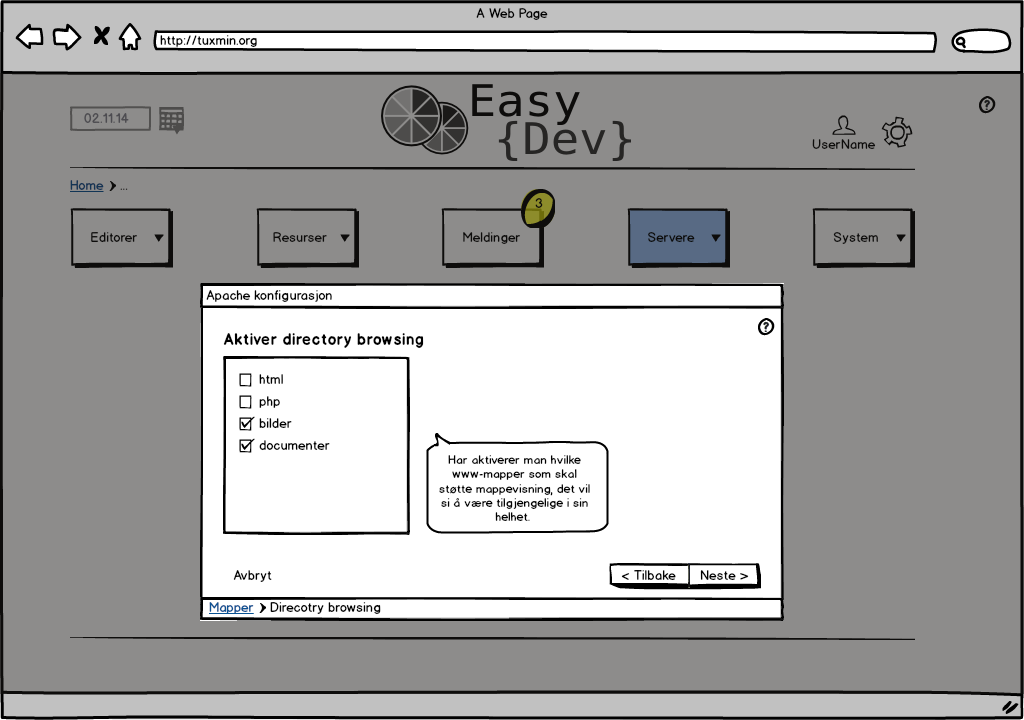
\includegraphics[width=\lowB\textwidth,height=\textheight,keepaspectratio]{./img/prosessdokumentasjon/lowfi/apache3.png}
\caption[Low-fi Webserver 3]{Webserver. Aktivering av <<directory browsing>>.}
\label{fig:apachelow3}
\end{figure}

\begin{figure}[ht]
\centering
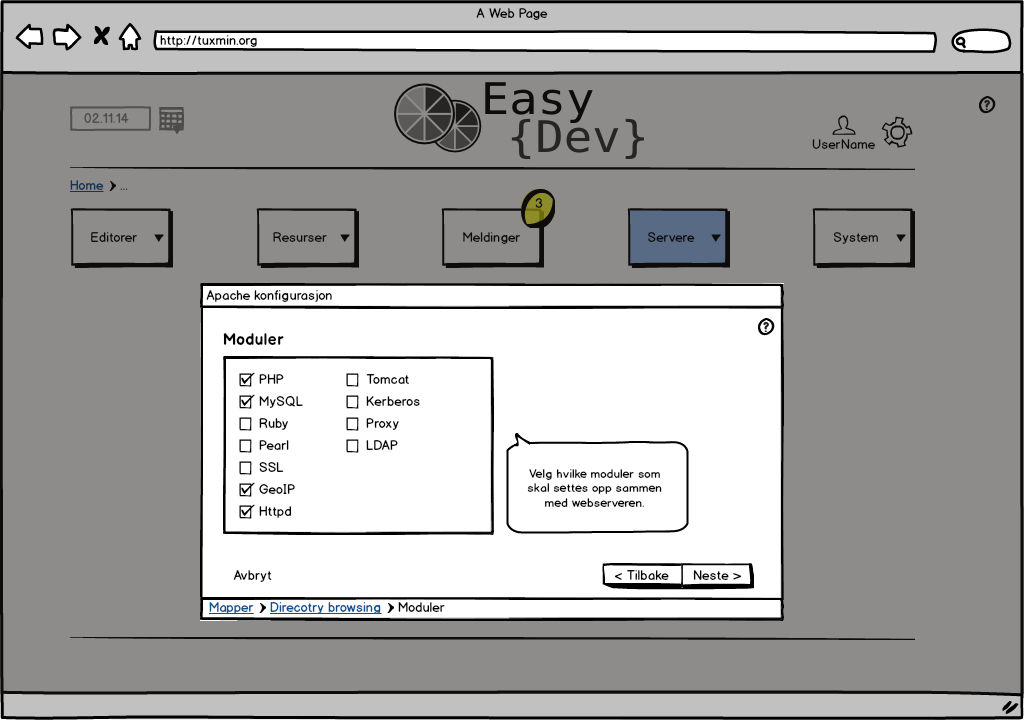
\includegraphics[width=\lowB\textwidth,height=\textheight,keepaspectratio]{./img/prosessdokumentasjon/lowfi/apache4.png}
\caption[Low-fi Webserver 4]{Webserver. Tillegsmoduler for webserver.}
\label{fig:apachelow4}
\end{figure}

\begin{figure}[ht]
\centering
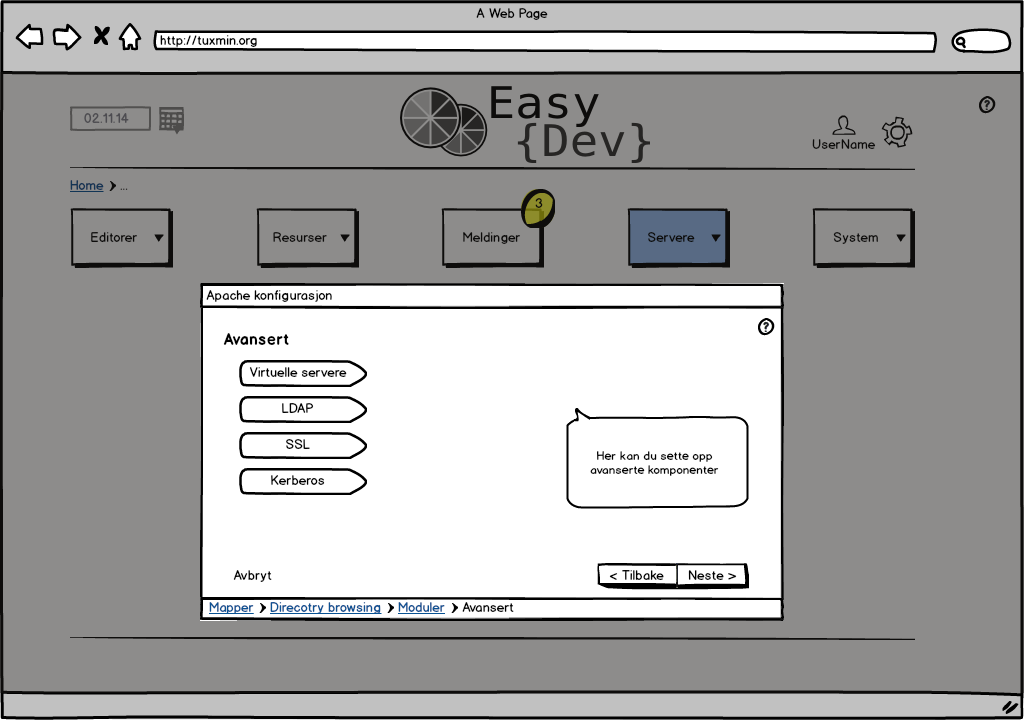
\includegraphics[width=\lowB\textwidth,height=\textheight,keepaspectratio]{./img/prosessdokumentasjon/lowfi/apache5.png}
\caption[Low-fi Webserver 5]{Webserver. Avanserte moduler.}
\label{fig:apachelow5}
\end{figure}

%KONFIGURASJON AV BRUKERE
\begin{figure}[ht]
\centering
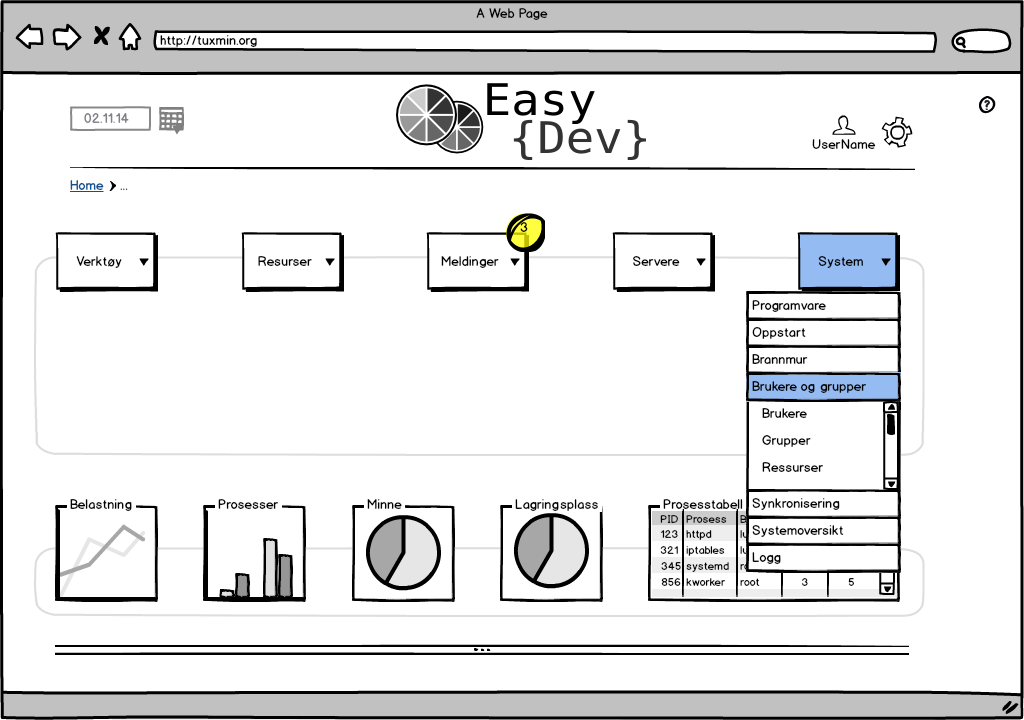
\includegraphics[width=\lowB\textwidth,height=\textheight,keepaspectratio]{./img/prosessdokumentasjon/lowfi/b1.png}
\caption[Low-fi Brukere 1]{Brukere. Aktivering av brukeradministrasjon skjer fra system modulen.}
\label{fig:brukerelow1}
\end{figure}

\begin{figure}[ht]
\centering
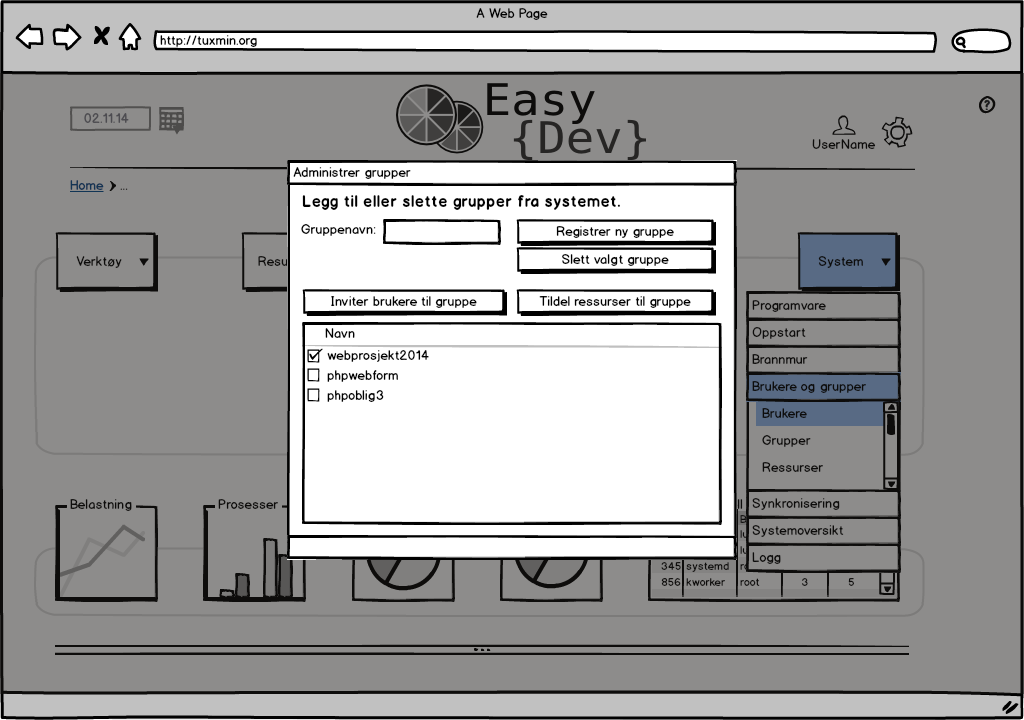
\includegraphics[width=\lowB\textwidth,height=\textheight,keepaspectratio]{./img/prosessdokumentasjon/lowfi/b2.png}
\caption[Low-fi Brukere 2]{Brukere. Administrasjon av grupper. Mulighet til å legge til nye grupper eller gå videre til brukerbehndling.}
\label{fig:brukerelow2}
\end{figure}

\begin{figure}[ht]
\centering
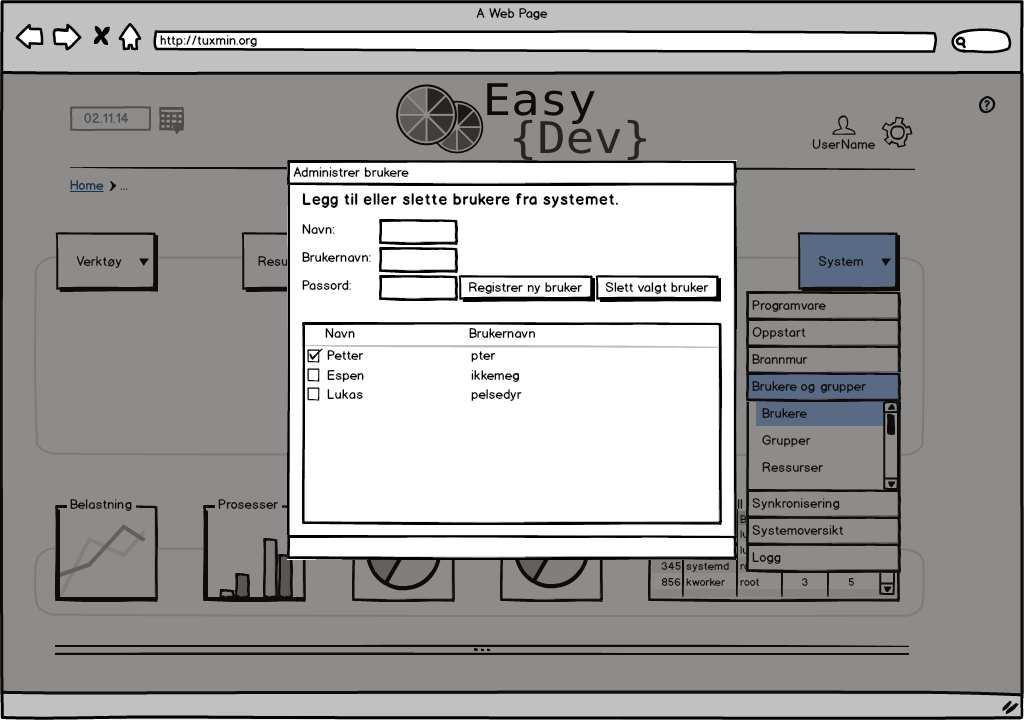
\includegraphics[width=\lowB\textwidth,height=\textheight,keepaspectratio]{./img/prosessdokumentasjon/lowfi/b3.png}
\caption[Low-fi Brukere 3]{Brukere. Administrasjon av brukere. Mulighet for å legge til eller slette brukere.}
\label{fig:brukerelow3}
\end{figure}

\begin{figure}[ht]
\centering
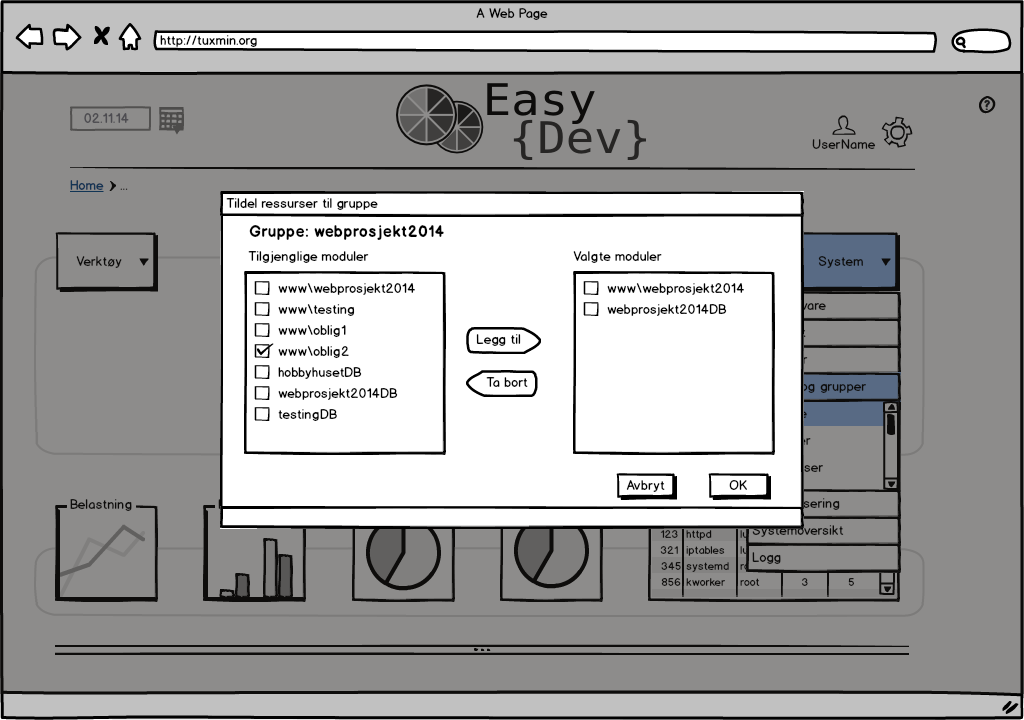
\includegraphics[width=\lowB\textwidth,height=\textheight,keepaspectratio]{./img/prosessdokumentasjon/lowfi/b4.png}
\caption[Low-fi Brukere 4]{Brukere. Val av moduler som de nye eller eksisterende grupper skal lha tilgang til. Det er også mulig å fjerne rettigheter fra grupper som fikk disse rettigheter tidligere.}
\label{fig:brukerelow4}
\end{figure}


%HIFI---------------------------------------------------
\section{Hi-fi prototype} \label{sec:appendiksHiFi}
\begin{figure}[ht]
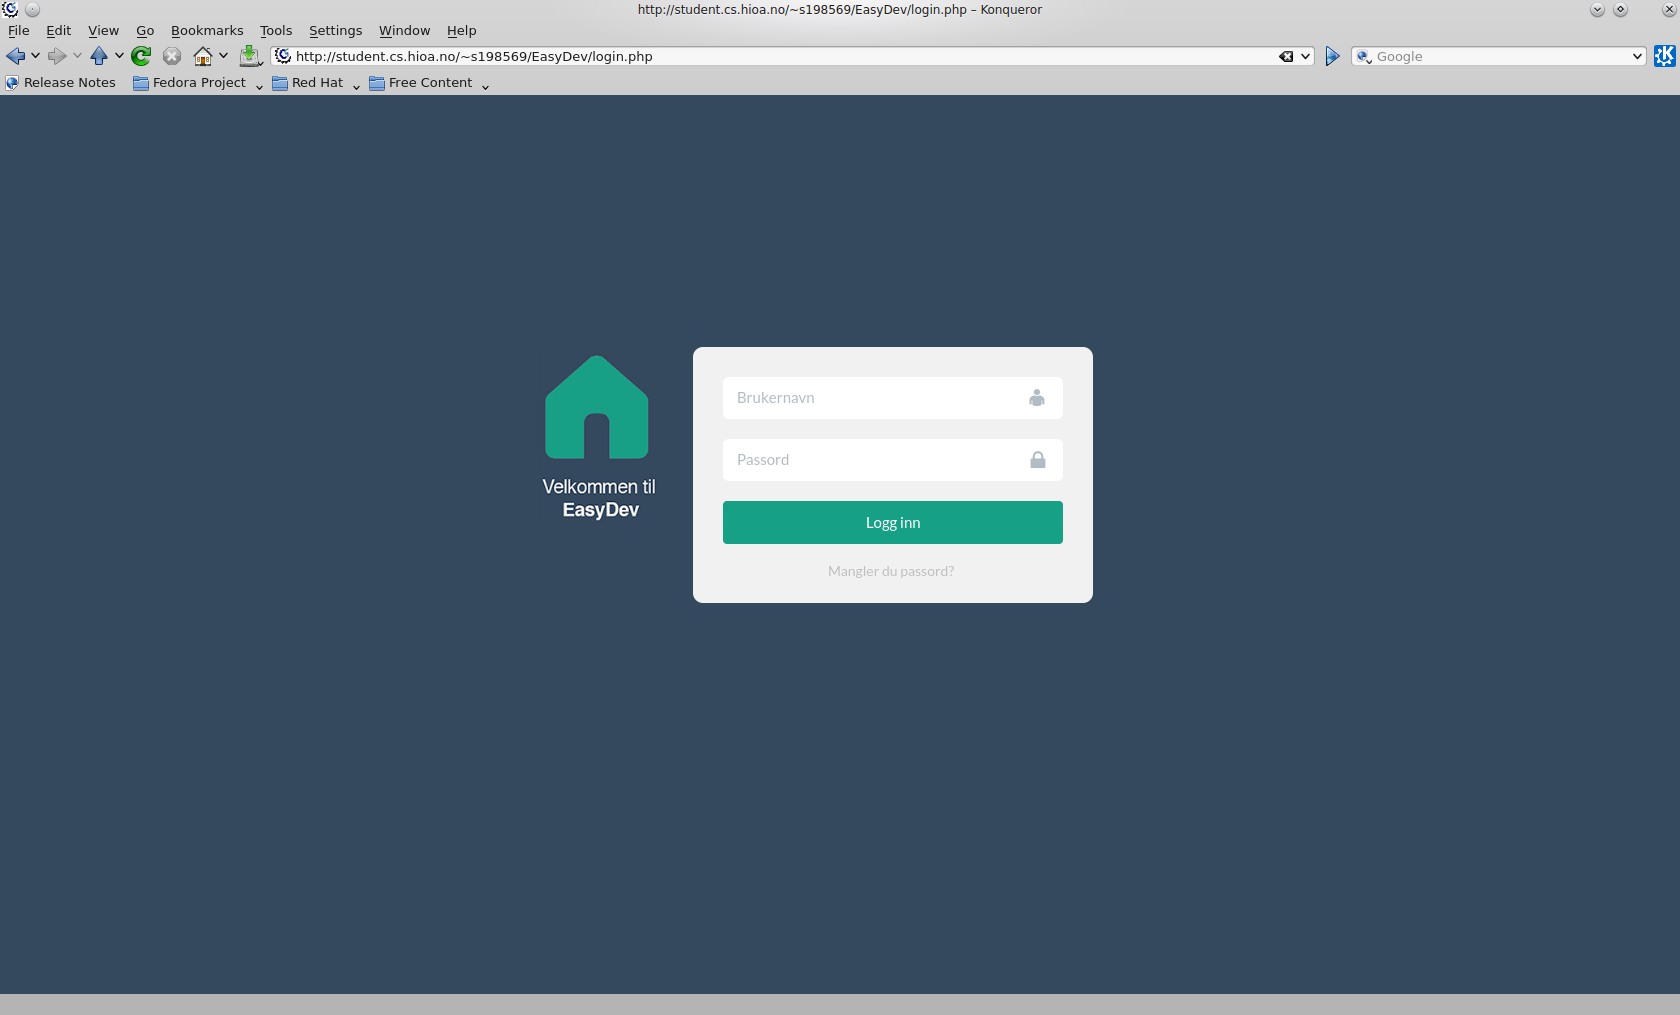
\includegraphics[width=\textwidth,height=\textheight,keepaspectratio]{./img/prosessdokumentasjon/hifi/login.png}
\caption[Hi-fi Påloggingsbilde]{Påloggingsbilde. I prtotypen er det mulig å logge seg på uten brukernavn eller passord. Etter dette påloggingsbilde blir brukeren forflyttet til fremside.}
\label{fig:loginhi}
\end{figure}

%KONFIGURASJON AV APACHE
\begin{figure}[ht]
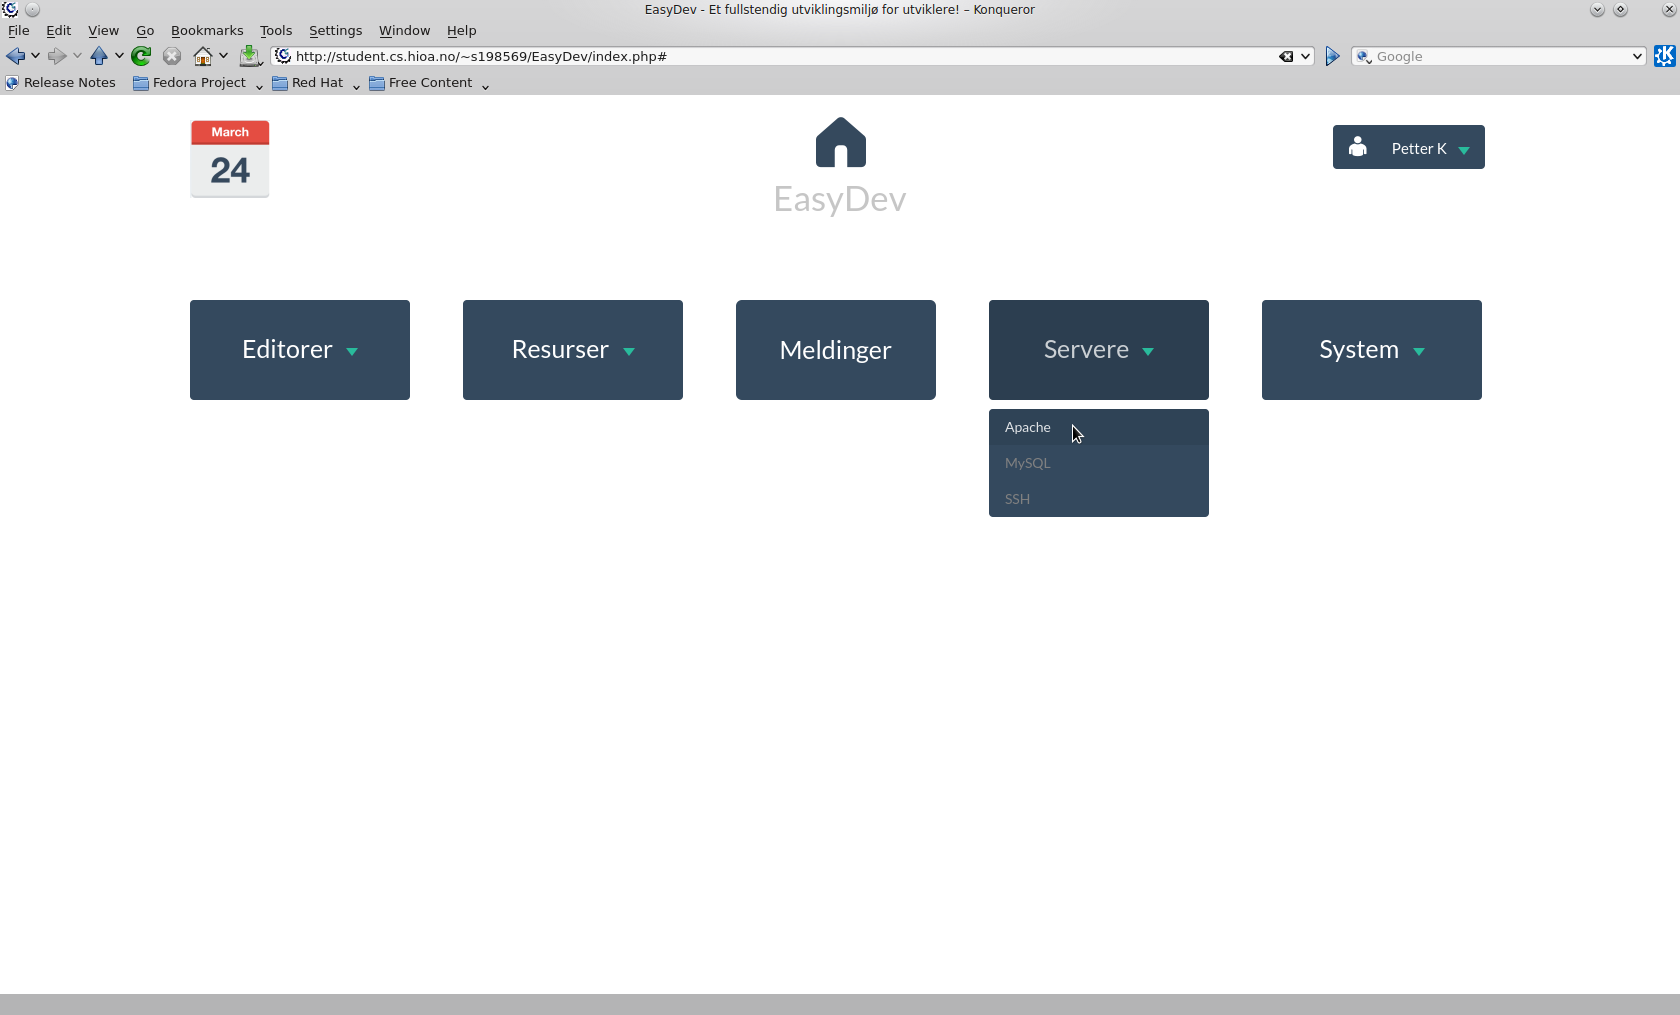
\includegraphics[width=\textwidth,height=\textheight,keepaspectratio]{./img/prosessdokumentasjon/hifi/a1.png}
\caption[Hi-fi Webserver 1]{Webserver. Her sakl brukeren sette igang konfigurasjon av webserver. Modulen for dette er logisk plassert under <<Servere>> kategorien.}
\label{fig:apachehi1}
\end{figure}

\begin{figure}[ht]
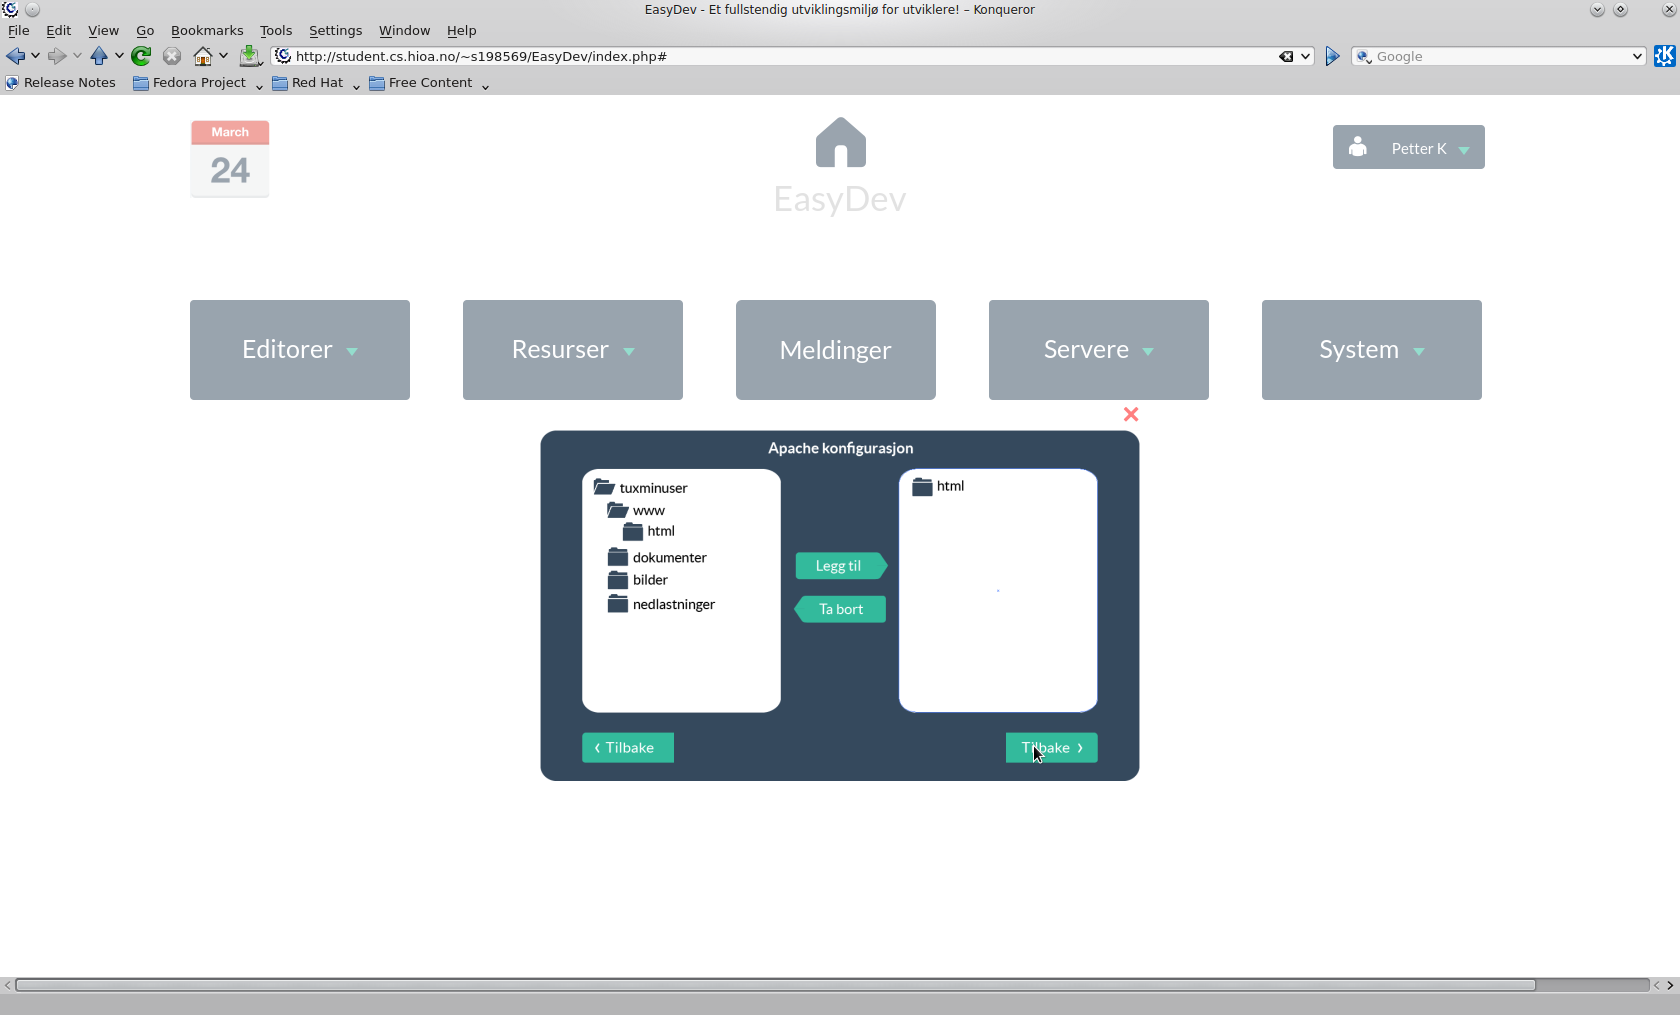
\includegraphics[width=\textwidth,height=\textheight,keepaspectratio]{./img/prosessdokumentasjon/hifi/a2.png}
\caption[Hi-fi Webserver 2]{Webserver. Valg av mapper som skal være konfigurert i webserveren.}
\label{fig:apachehi2}
\end{figure}

\begin{figure}[ht]
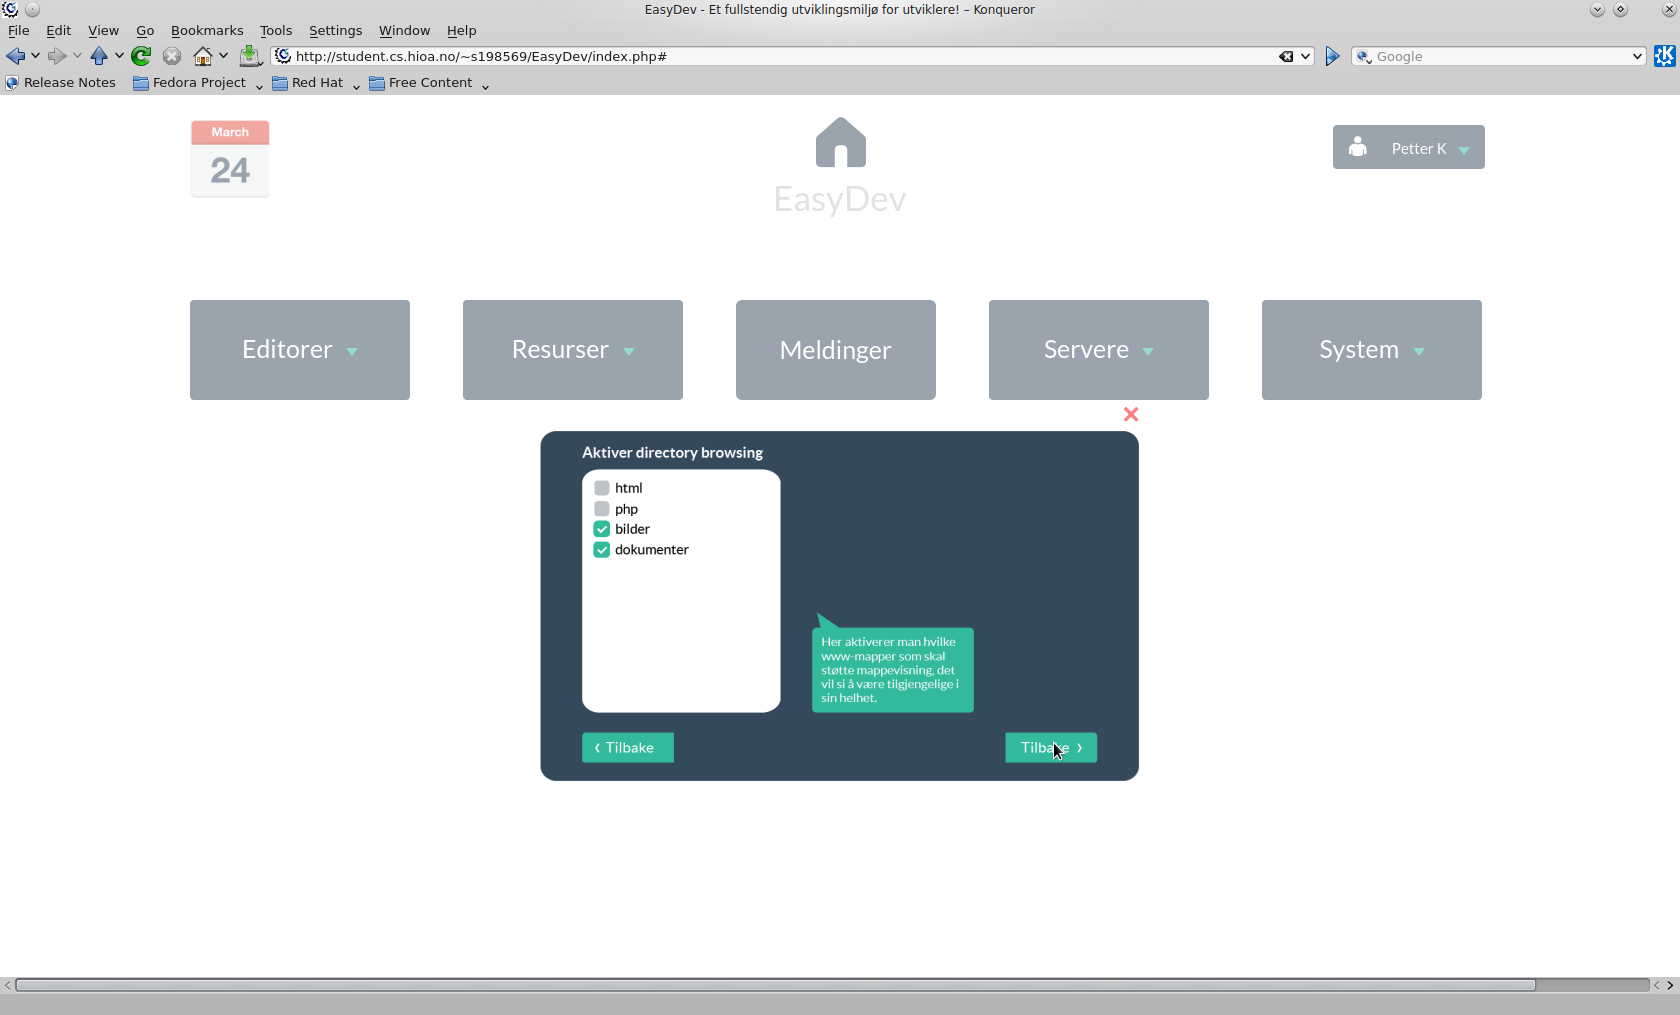
\includegraphics[width=\textwidth,height=\textheight,keepaspectratio]{./img/prosessdokumentasjon/hifi/a3.png}
\caption[Hi-fi Webserver 3]{Webserver. Aktivering av <<directory browsing>>.}
\label{fig:apachehi3}
\end{figure}

\begin{figure}[ht]
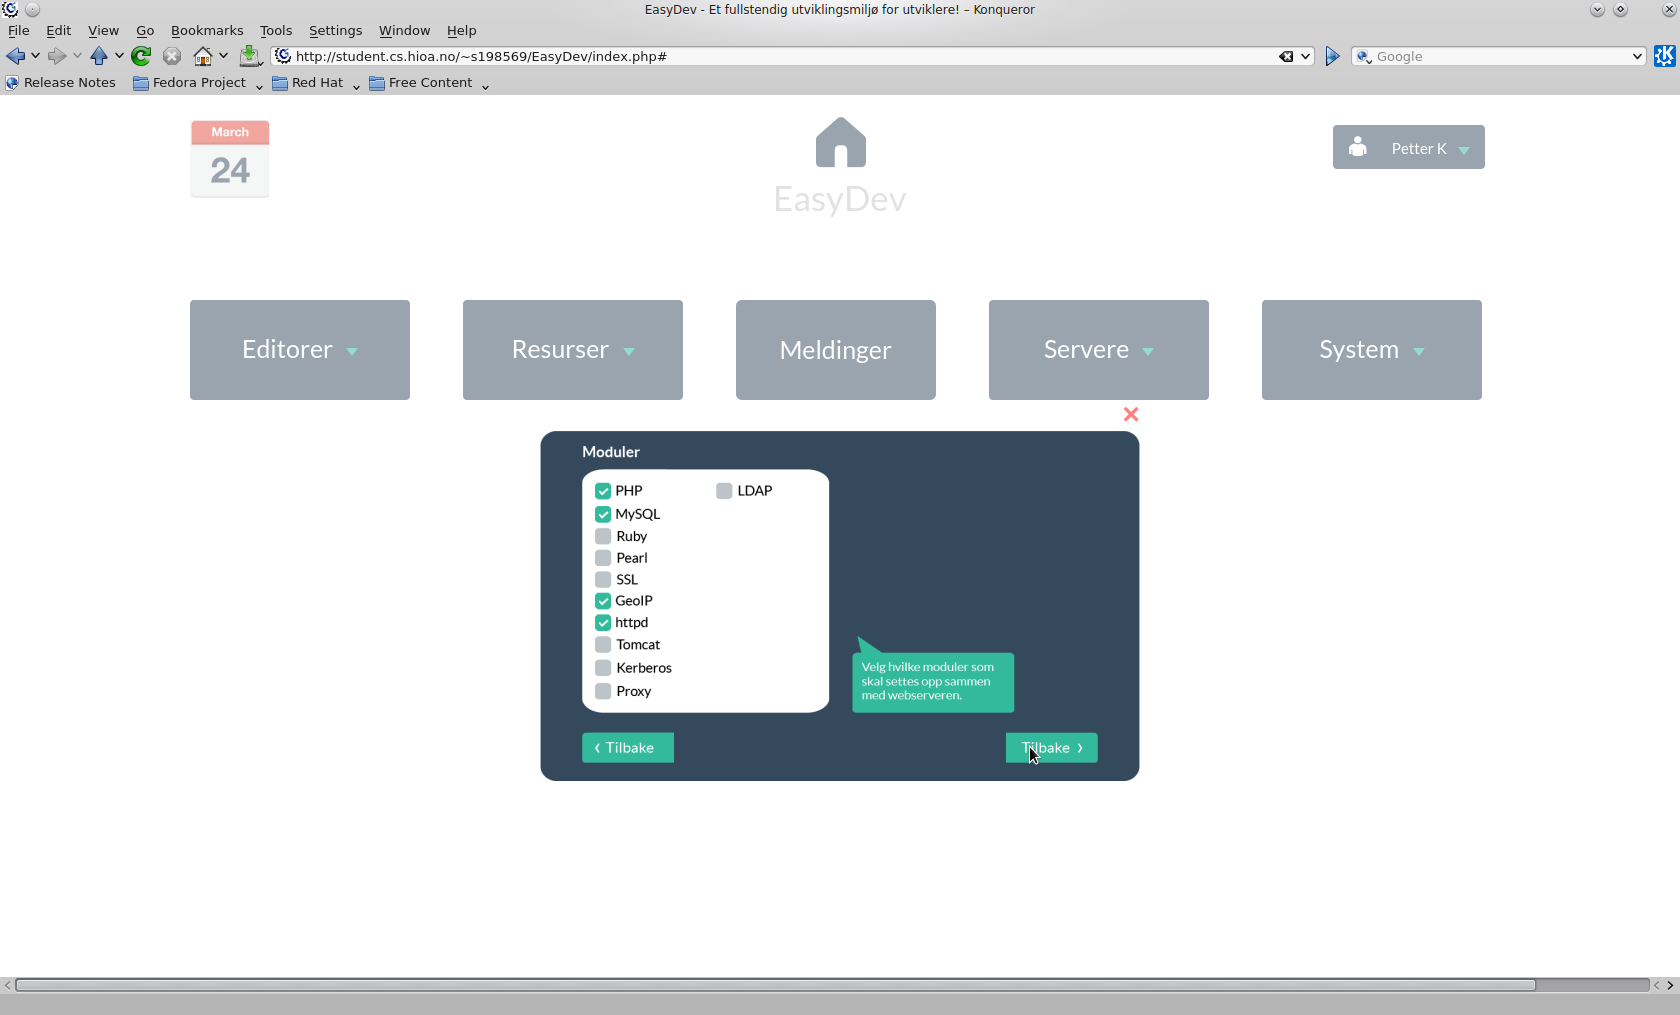
\includegraphics[width=\textwidth,height=\textheight,keepaspectratio]{./img/prosessdokumentasjon/hifi/a4.png}
\caption[Hi-fi Webserver 4]{Webserver. Tillegsmoduler for webserver.}
\label{fig:apachehi4}
\end{figure}

\begin{figure}[ht]
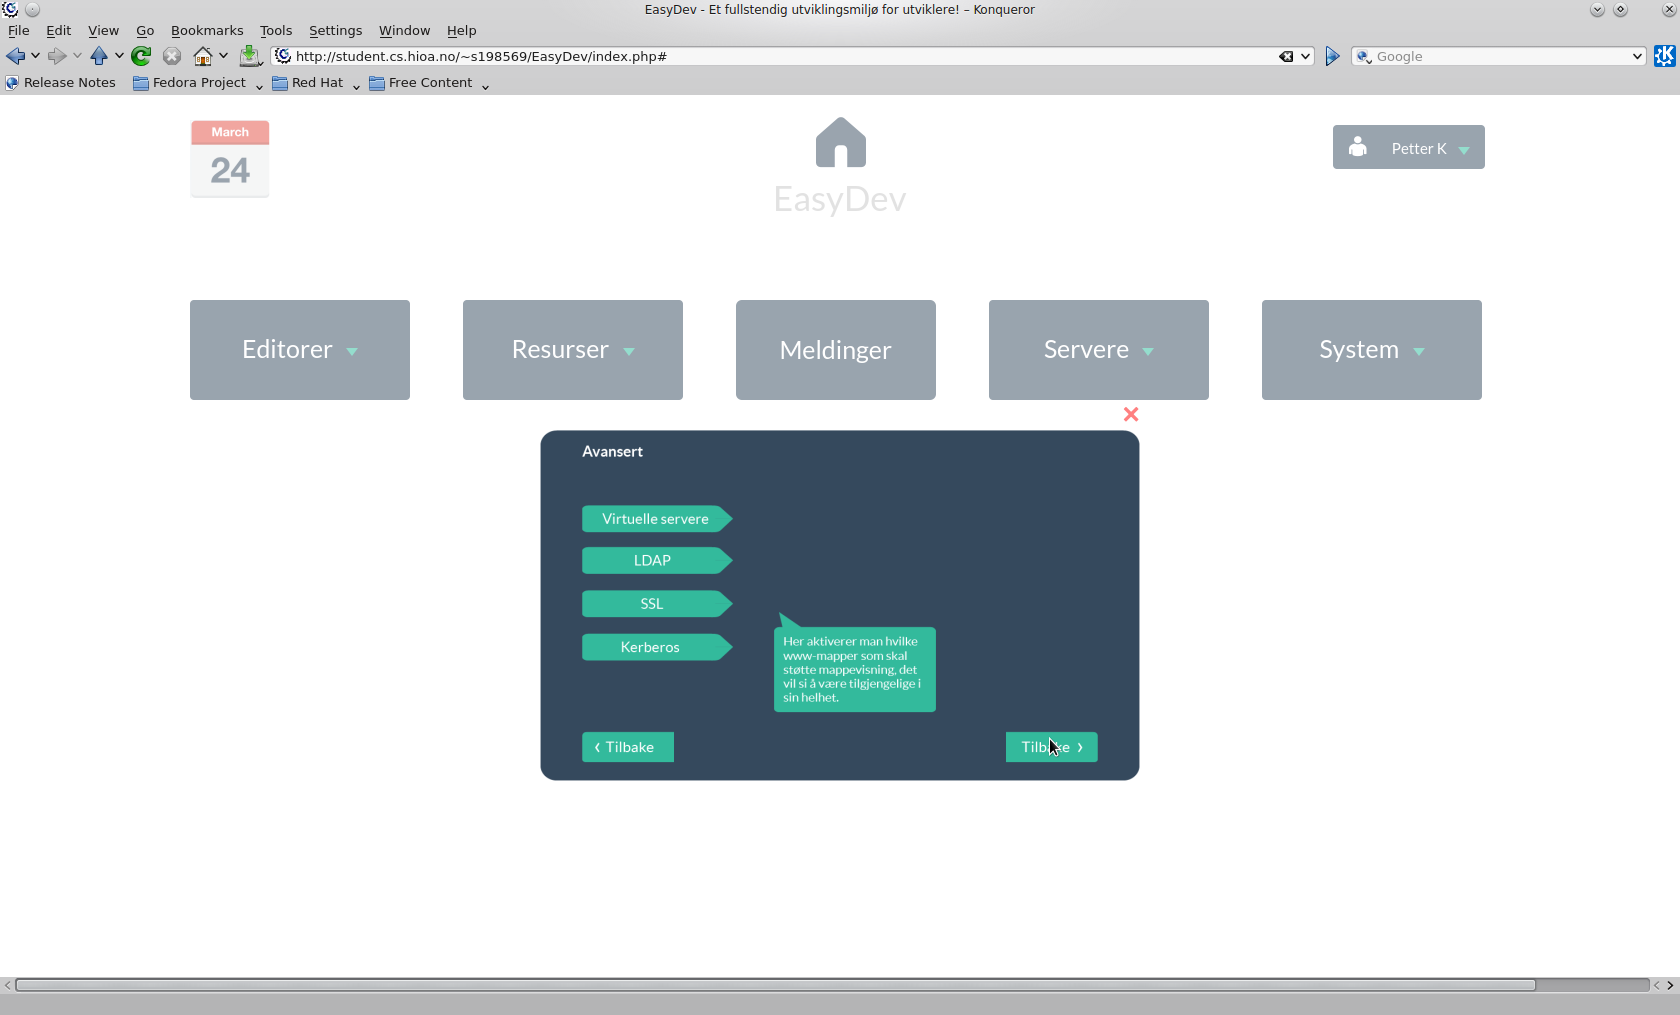
\includegraphics[width=\textwidth,height=\textheight,keepaspectratio]{./img/prosessdokumentasjon/hifi/a5.png}
\caption[Hi-fi Webserver 5]{Webserver. Avanserte moduler.}
\label{fig:apachehi5}
\end{figure}

%KONFIGURASJON AV BRUKERE
\begin{figure}[ht]
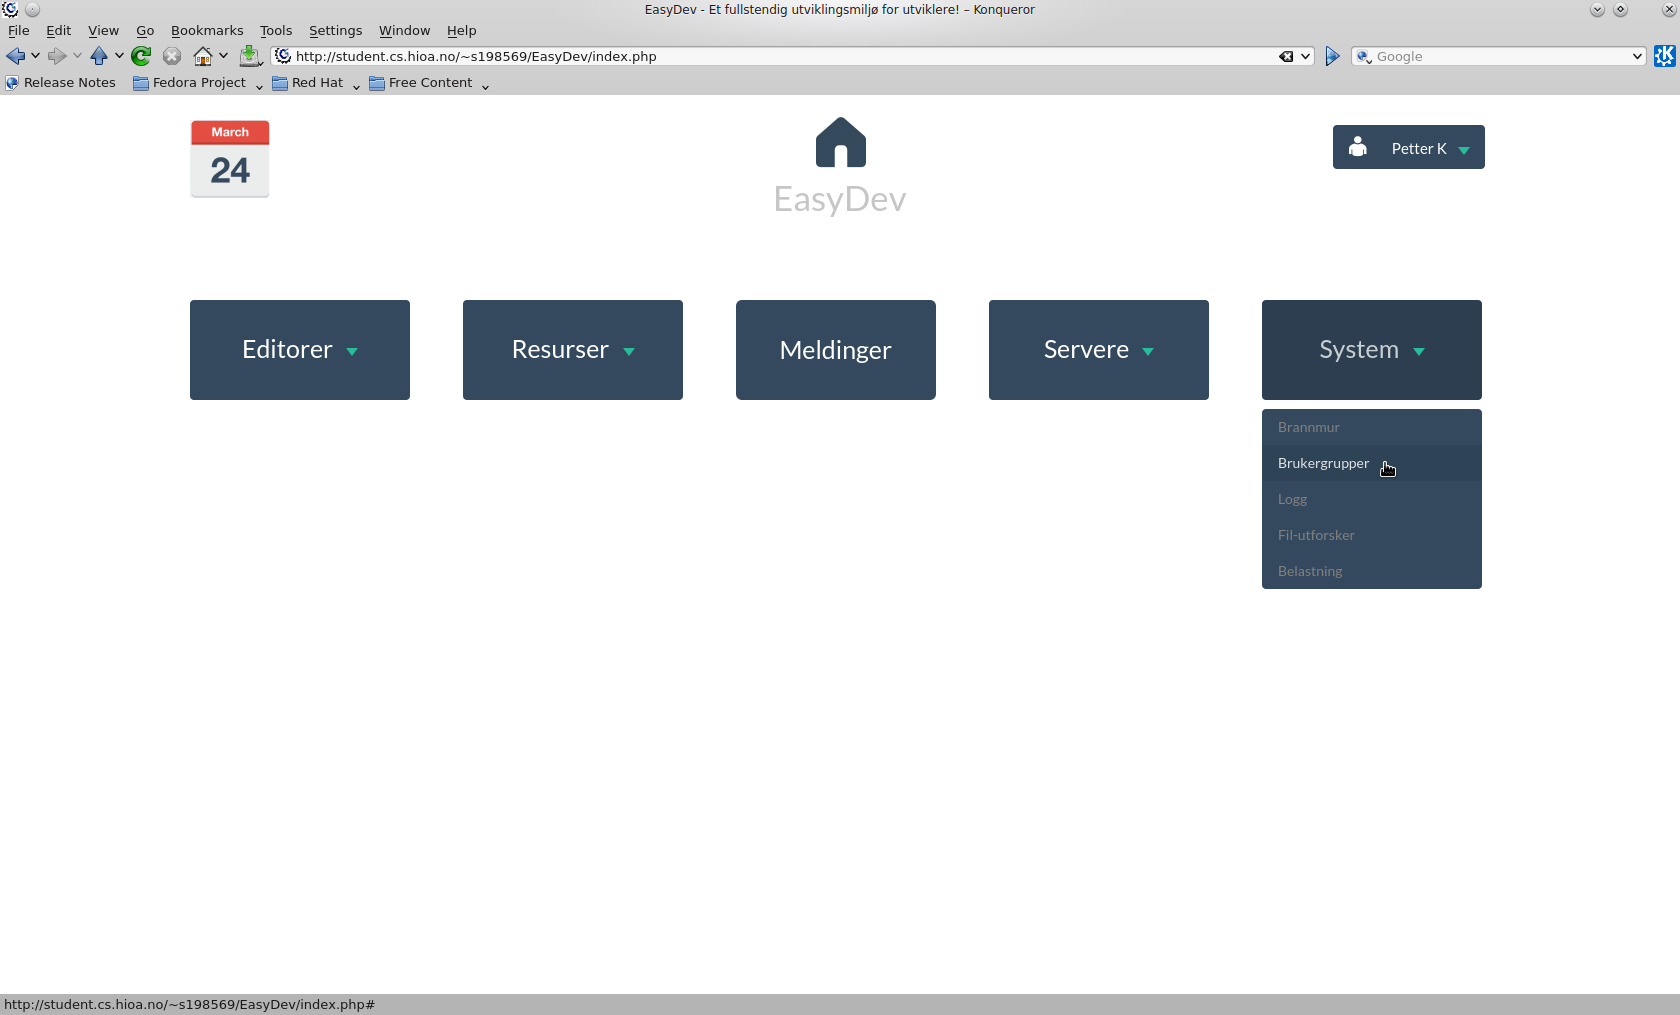
\includegraphics[width=\textwidth,height=\textheight,keepaspectratio]{./img/prosessdokumentasjon/hifi/b1.png}
\caption[Hi-fi Brukere 1]{Brukere. Aktivering av brukeradministrasjon skjer fra system modulen.}
\label{fig:brukerehi1}
\end{figure}

\begin{figure}[ht]
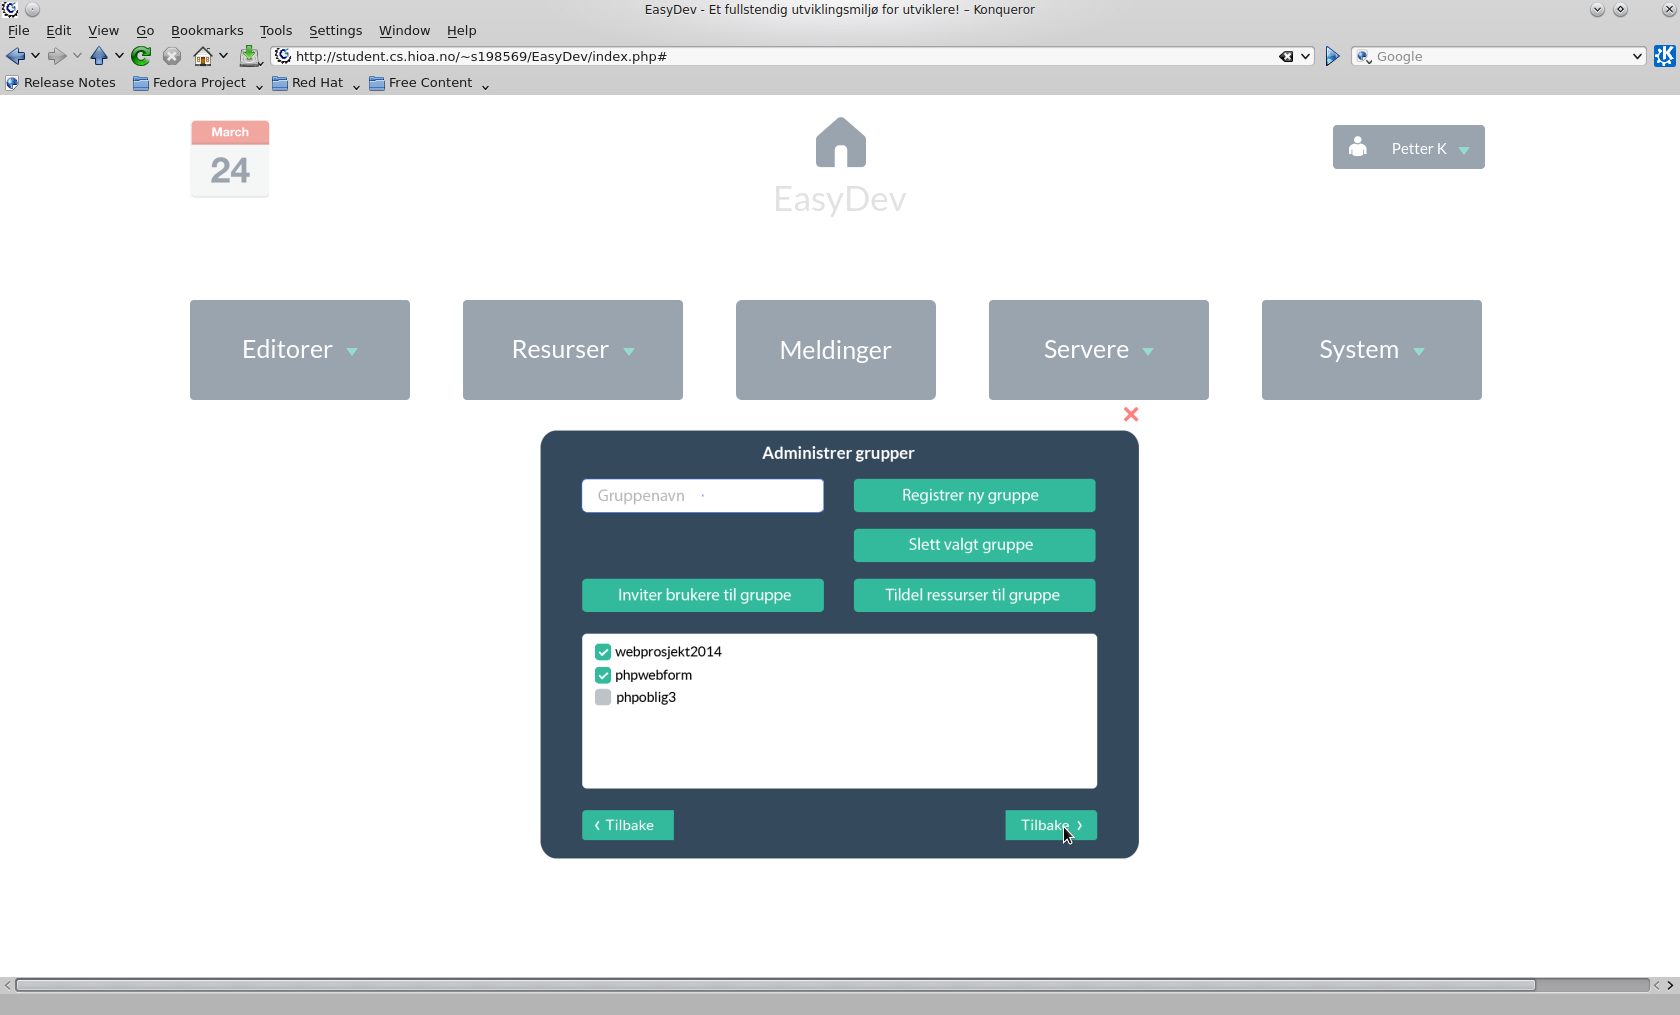
\includegraphics[width=\textwidth,height=\textheight,keepaspectratio]{./img/prosessdokumentasjon/hifi/b2.png}
\caption[Hi-fi Brukere 2]{Brukere. Administrasjon av grupper. Mulighet til å legge til nye grupper eller gå videre til brukerbehndling.}
\label{fig:brukerehi2}
\end{figure}

\begin{figure}[ht]
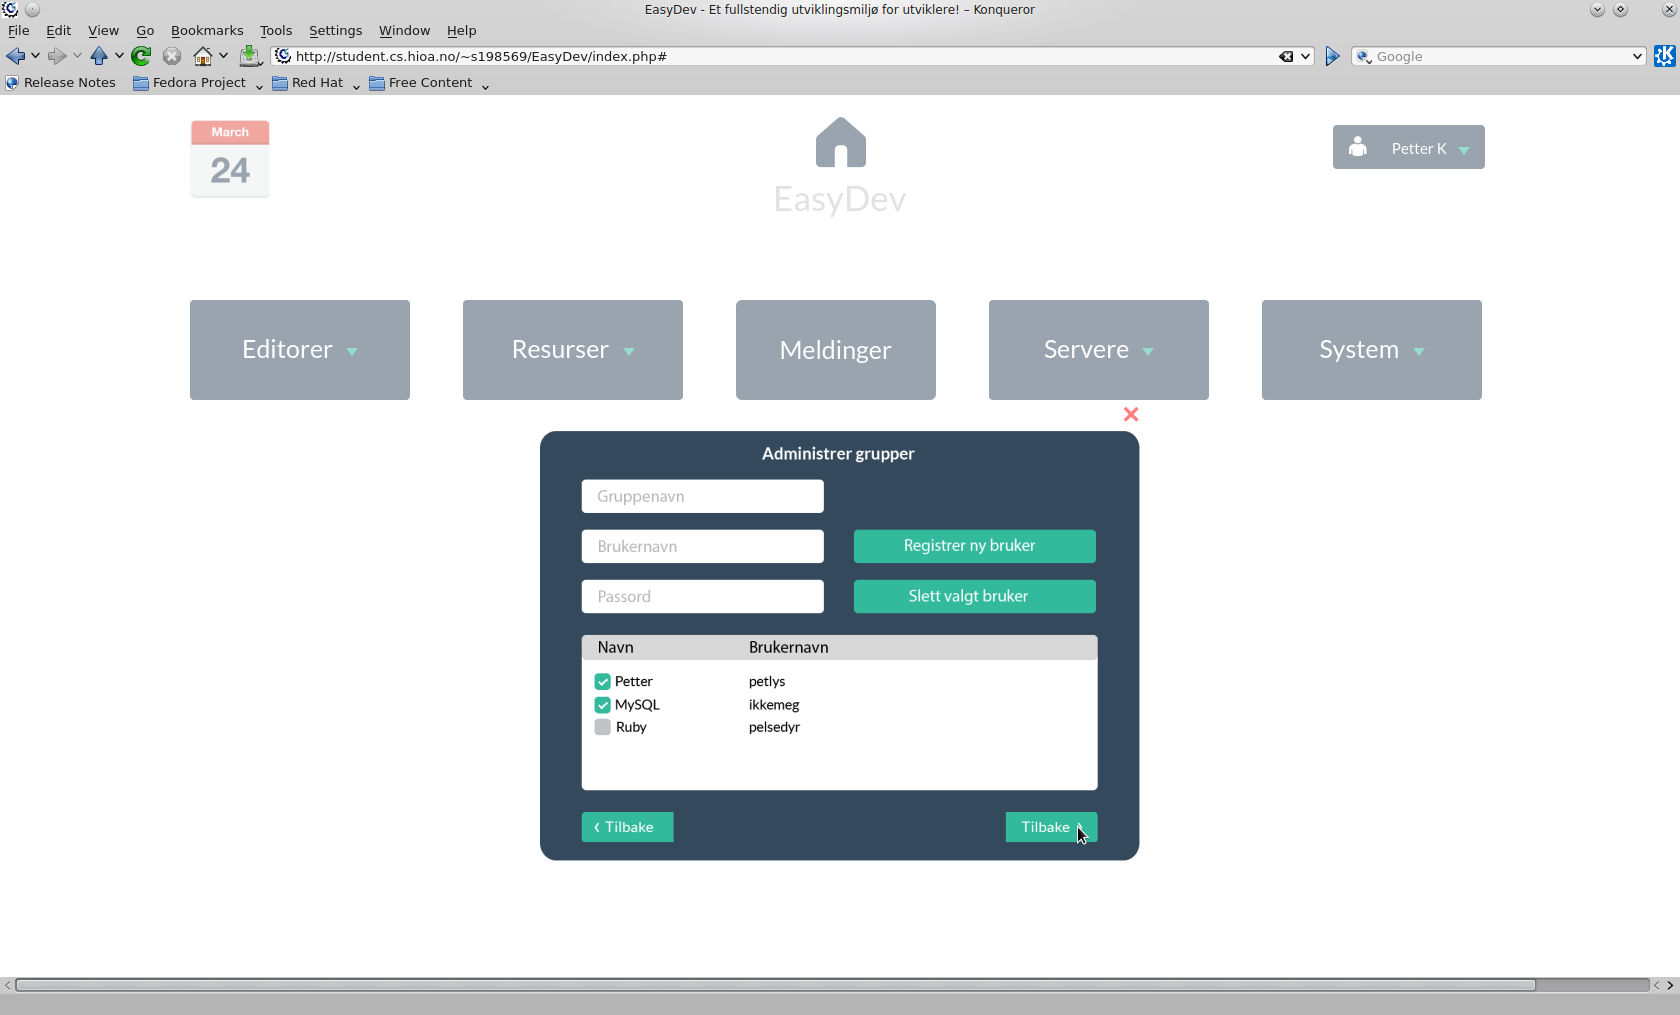
\includegraphics[width=\textwidth,height=\textheight,keepaspectratio]{./img/prosessdokumentasjon/hifi/b3.png}
\caption[Hi-fi Brukere 3]{Brukere. Administrasjon av brukere. Mulighet for å legge til eller slette brukere.}
\label{fig:brukerehi3}
\end{figure}

\begin{figure}[ht]
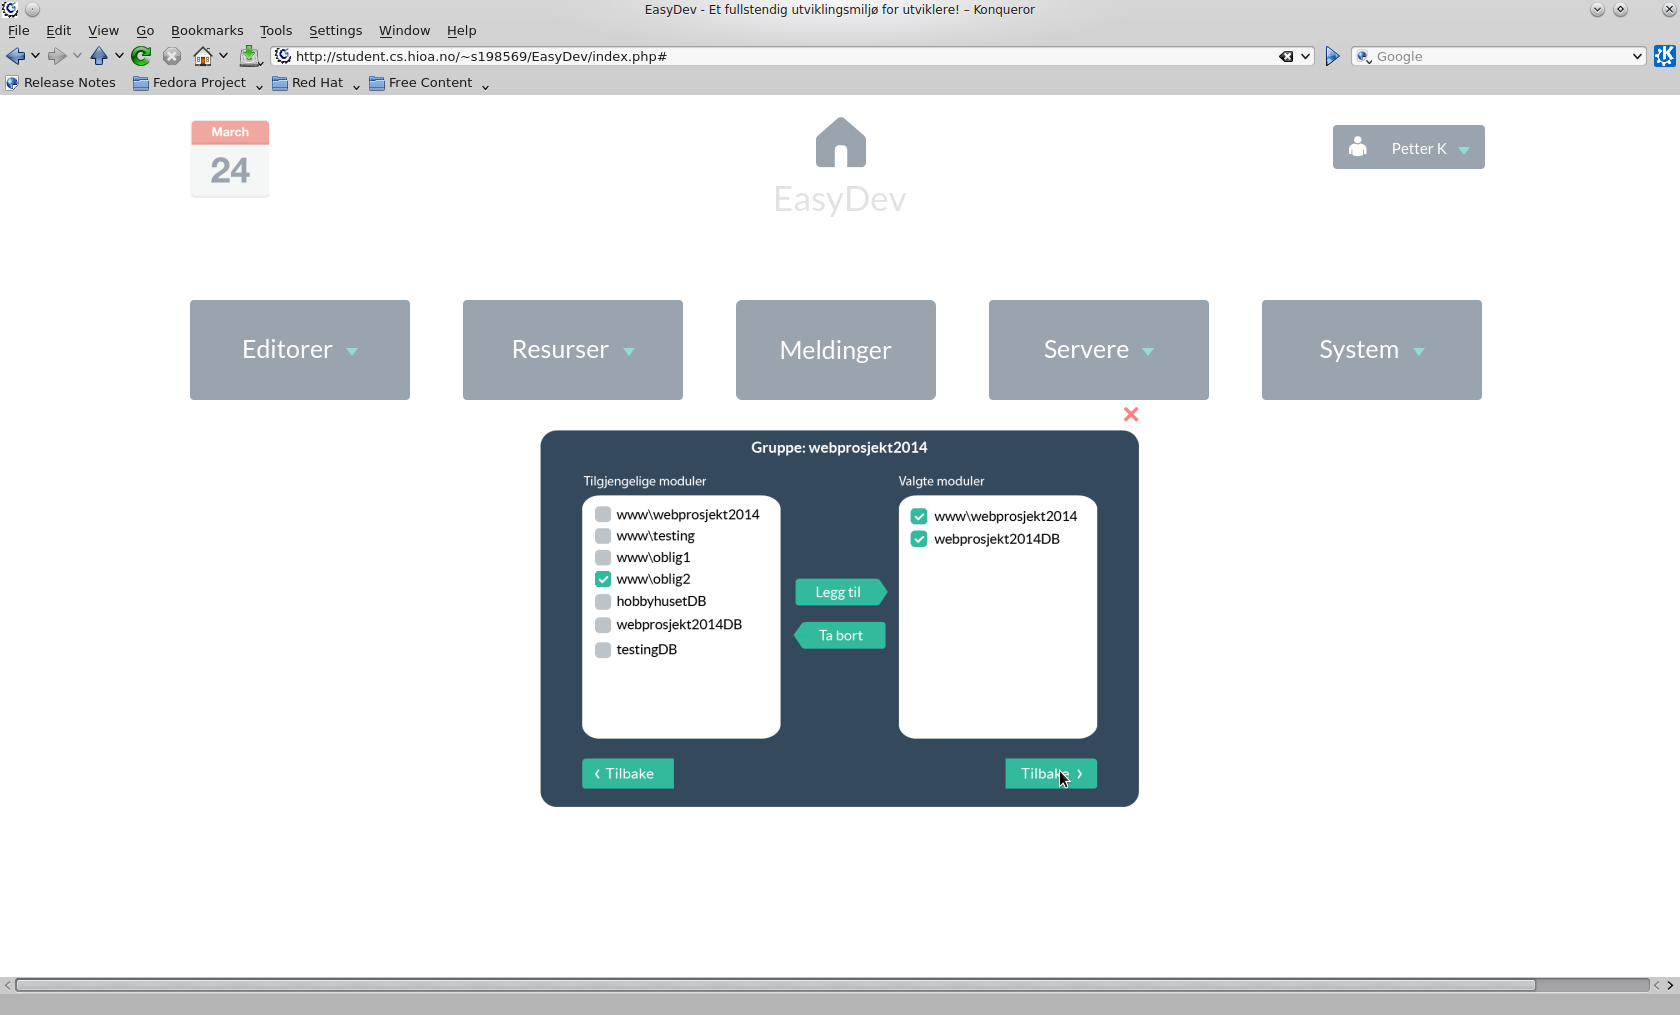
\includegraphics[width=\textwidth,height=\textheight,keepaspectratio]{./img/prosessdokumentasjon/hifi/b4.png}
\caption[Hi-fi Brukere 4]{Brukere. Val av moduler som de nye eller eksisterende grupper skal lha tilgang til. Det er også mulig å fjerne rettigheter fra grupper som fikk disse rettigheter tidligere.}
\label{fig:brukerehi4}
\end{figure}